\documentclass{beamer}

\mode<presentation> {

% The Beamer class comes with a number of default slide themes
% which change the colors and layouts of slides. Below this is a list
% of all the themes, uncomment each in turn to see what they look like.

%\usetheme{default}
%\usetheme{AnnArbor}
%\usetheme{Antibes}
%\usetheme{Bergen}
%\usetheme{Berkeley}
%\usetheme{Berlin}
%\usetheme{Boadilla}
\usetheme{CambridgeUS}
%\usetheme{Copenhagen}
%\usetheme{Darmstadt}
%\usetheme{Dresden}
%\usetheme{Frankfurt}
%\usetheme{Goettingen}
%\usetheme{Hannover}
%\usetheme{Ilmenau}
%\usetheme{JuanLesPins}
%\usetheme{Luebeck}
%\usetheme{Madrid}
%\usetheme{Malmoe}
%\usetheme{Marburg}
%\usetheme{Montpellier}
%\usetheme{PaloAlto}
%\usetheme{Pittsburgh}
%\usetheme{Rochester}
%\usetheme{Singapore}
%\usetheme{Szeged}
%\usetheme{Warsaw}

% As well as themes, the Beamer class has a number of color themes
% for any slide theme. Uncomment each of these in turn to see how it
% changes the colors of your current slide theme.

%\usecolortheme{albatross}
%\usecolortheme{beaver}
%\usecolortheme{beetle}
%\usecolortheme{crane}
%\usecolortheme{dolphin}
%\usecolortheme{dove}
%\usecolortheme{fly}
%\usecolortheme{lily}
%\usecolortheme{orchid}
%\usecolortheme{rose}
%\usecolortheme{seagull}
%\usecolo rtheme{seahorse}
%\usecolortheme{whale}
%\usecolortheme{wolverine}

%\setbeamertemplate{footline} % To remove the footer line in all slides uncomment this line
%\setbeamertemplate{footline}[page number] % To replace the footer line in all slides with a simple slide count uncomment this line

%\setbeamertemplate{navigation symbols}{} % To remove the navigation symbols from the bottom of all slides uncomment this line
}

\usepackage{graphicx} % Allows including images
\usepackage{booktabs} % Allows the use of \toprule, \midrule and \bottomrule in tables
%\usepackage{german}
\usepackage{braket}
\usepackage{bbold}
\usepackage[utf8]{inputenc}
\usepackage{wasysym}
\usepackage{hyperref}
\usepackage{tcolorbox}
\usepackage{ragged2e}
%----------------------------------------------------------------------------------------
%	TITLE PAGE
%----------------------------------------------------------------------------------------

\title[HPC 1b]{High Performance Computing 1b \\
Parallelization of a 2D Hydro Solver} % The short title appears at the bottom of every slide, the full title is only on the title page

\author[Hertig, Radonic]{Remo Hertig\\
Stephan Radonic} % Your name
\institute[UZH] % Your institution as it will appear on the bottom of every slide, may be shorthand to save space
{
University of Zurich
}
\date{\today} % Date, can be changed to a custom date

\begin{document}

\begin{frame}
\titlepage % Print the title page as the first slide
\end{frame}

%\begin{frame}
%\frametitle{Overview} % Table of contents slide, comment this block out to remove it
%\tableofcontents % Throughout your presentation, if you choose to use \section{} and \subsection{} commands, these will automatically be printed on this slide as an overview of your presentation
%\end{frame}

%----------------------------------------------------------------------------------------
%	PRESENTATION SLIDES
%----------------------------------------------------------------------------------------

%------------------------------------------------
%\section{HYDRO Parallelization} % Sections can be created in order to organize your presentation into discrete blocks, all sections and subsections are automatically printed in the table of contents as an overview of the talk
%------------------------------------------------
%\subsection{Introduction}
%\subsection{Parallelization strategy}
%\subsection{Serial vs. Parallel Processing}
%\subsection{Scaling and Speedup}
%\subsection{High resolution example}
%
%
%
\begin{frame}
\frametitle{Introduction and physics}
\justify
\small{
Our task was to parallelize an existing C code, originally written by Prof. Romain Teyssier in Fortran, which solves the Euler equations in 2D using a Godunov scheme. The euler equations in conservation form are 
\begin{equation}
\partial_t
\begin{pmatrix} \rho    \\ \rho \mathbf{u}\\0\end{pmatrix}+\nabla\cdot\begin{pmatrix} \rho\mathbf{u}    \\ \rho\mathbf{u}\otimes\mathbf{u}+p\mathbf{I}\\ \mathbf{u}\end{pmatrix} = 0
\end{equation}
This set of equations describes the flow of a gas basically stating the momentum, mass and energy conservation. A hyperbolic PDE in conservation law form is generally represented as
\begin{equation}
\partial_t\mathbf{U} + \nabla\cdot\mathbf{F(U)} = 0
\label{eq:bb}
\end{equation}
Discretization on a grid yields
\begin{equation}
\mathbf{U}^{n+1}_i=\mathbf{U^n_i}+\frac{\Delta x}{\Delta t}(\mathbf{F_{i-1/2}}-\mathbf{F_{i+1/2}})
\label{eq:bc}
\end{equation}
where $\mathbf{F_{i\pm1/2}}$ are the fluxes at the cell boundaries, the Godunov scheme uses various approximations for $\mathbf{F_{i\pm1/2}}$, depending on the specific variation of the method, e.g upwind scheme, lax-friedrich, ... \\
}
\\
\vspace{1mm}

\end{frame}
%
%
%
\begin{frame}
\frametitle{Parallelization}

We implemented a symetric vertical domain decomposition\footnote{ 
\emph{Restriction: $Width=\{n_{proc}k|k\in\mathbb{N}\}$ } } and used nonblocking MPI communication to share ghost cells.\\

Since the resulting data output is massive (\textasciitilde{}600Mb for a 10M grid per step) it is currently unpractical to store the results from every step. Therefore we opted for a lower storage resolution. This allows us to implement the "write-to-disk" part in a rather sub-optimal way: MPI\_Gather to the master. However the performance impact of this strategy is negligible over a long simulation time.\\

 


\end{frame}

\begin{frame}
\frametitle{Exploratory runs}

\end{frame}


%
%
%
\begin{frame}
\frametitle{Parallelization: Speedup and Scaling}
\justify
We compare the average time step durations for a single process up to approximatly 1500 parallel processses for a fixed problem size (in our case 60994 x 120). As observable in the strong scaling graph (ref figure) we get a super linear scaling up to 800 processes. 
The super linearity of the scaling can be explained with cache usage effects. \\
\vspace{2mm}
Oprimal cache memory usage only works well for rectangular shaped domains (large x small y for parallelization in x direction). We have compared how a fixed sized problem performs with diffrent $x/y$ ratios (see figure xx). We can cleary see that the performance increases with deacrasing $y/x$ size, up to a ratio, where each processes computing domain gets too small and becomes inefficient. 
\end{frame}
%
%
%
\begin{frame}
\frametitle{Parallelization: Speedup and Scaling}
\begin{minipage}[1\textheight]{\textwidth}
\begin{columns}[T]
\begin{column}{0.5\textwidth}
\begin{figure}
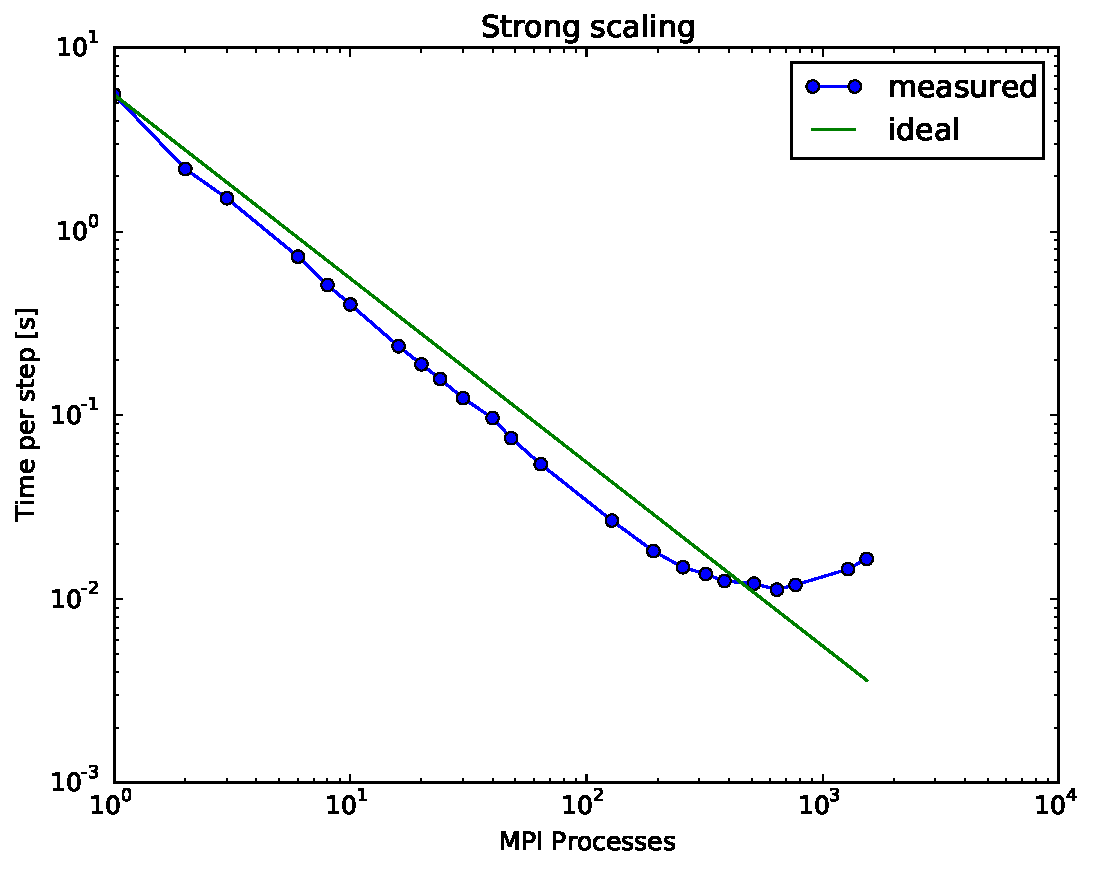
\includegraphics[width=6.75cm]{strongscale.pdf}
\caption{Strong scaling for a fixed grid size of $69994\times 120$ for 1 to 1536 processes. with the time step decreasing from 4.65 to 0.009}
\end{figure}
\end{column}


\begin{column}{0.5\textwidth}
\begin{figure}
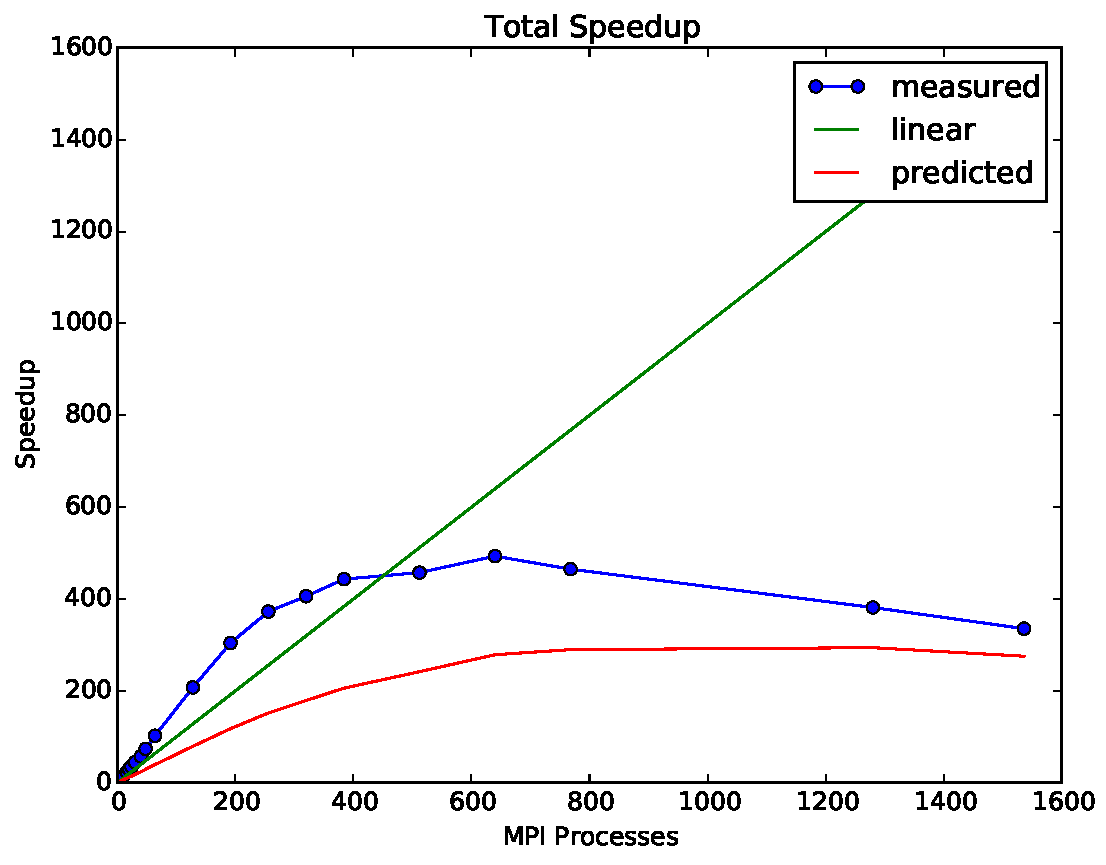
\includegraphics[width=6.75cm]{speedup.pdf}
\caption{Performance comparison of a fixed sized grid with varinyg $y/x$ ratio}
\end{figure}
\end{column}
\end{columns}
\end{minipage}
\end{frame}
%
%
%
\begin{frame}
\frametitle{Parallelization: Speedup and Scaling}
\begin{minipage}[1\textheight]{\textwidth}
\begin{columns}[T]
\begin{column}{0.5\textwidth}
\vspace{5mm}
\justify
...tzututzut
\end{column}
\begin{column}{0.5\textwidth}
\begin{figure}
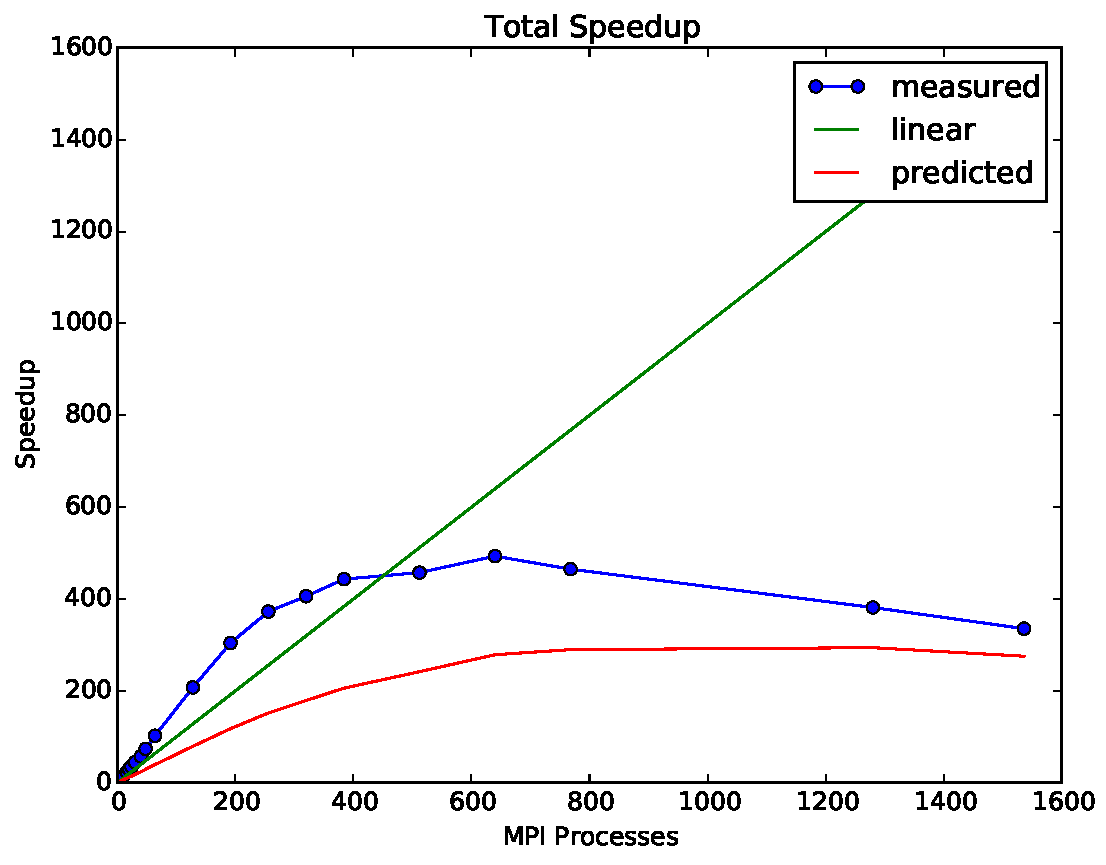
\includegraphics[width=6cm]{speedup.pdf}
\caption{}
\end{figure}
\end{column}
\end{columns}
\end{minipage}
\end{frame}
%
%
%
\begin{frame}
\frametitle{Output image}
\justify
To show the power of parallel processing we wanna show an excerpt from our high resolution image (3060 x 500) at simulation time t=600 seconds (corresponds to the 200'000th time step in our simulation). In order to avoid unnecessary wasting of computing resources, we didn't want to use a larger grid size. 
\begin{figure}
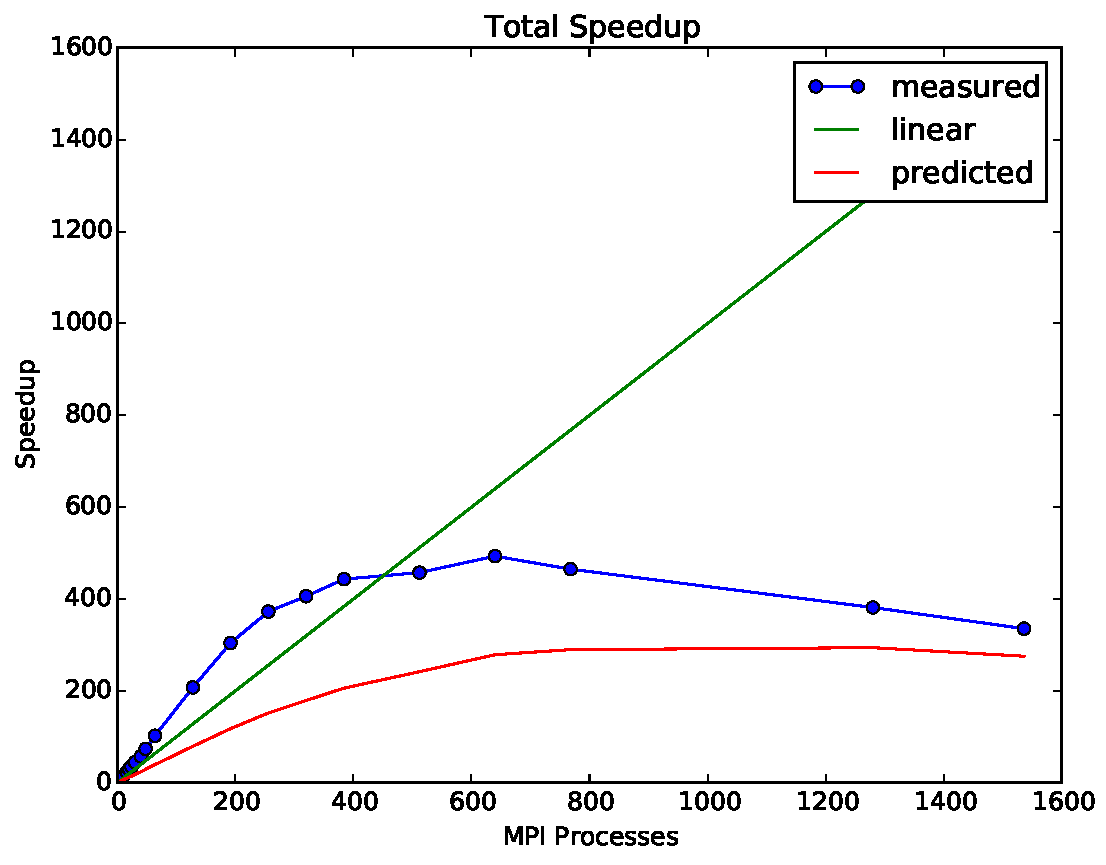
\includegraphics[width=12cm]{speedup.pdf}
\end{figure}
\end{frame}
%
%
%
\end{document} 
